\documentclass[10pt,letterpaper]{article}
\usepackage{graphicx}
\usepackage[utf8]{inputenc}
\usepackage[spanish]{babel} 
\usepackage{amsmath}
\usepackage{amsfonts}
\usepackage{amssymb}
\usepackage{fullpage}




\begin{document}
\begin{titlepage}
\begin{minipage}{12cm} Universidad de Chile
\\ Facultad de Ciencias F\'isicas y Matem\'aticas
\\ Departamento de Ciencias de la Computaci\'on\\
\\
\end{minipage}
\vspace*{2cm}
\begin{center}
\vspace{0.2cm}
{\Large \bf\vspace{0.5cm} Informe de Trabajo Dirigido}\\
{\Huge\bf\vspace{0.3cm} Tripdroid:}\\
{\Huge\bf\vspace{0.3cm} Georreferenciación Colaborativa}\\
{\Huge\bf\vspace{0.2cm} en Dispositivos Móviles}\\

\end{center}
\vspace{4cm}
\begin{tabular}{ll}
\bf{Nombre Alumno :}& Jorge Romo J. \\
\bf{Carrera:} & Ingeniería Civil en Computación\\ 
\bf{Profesor:} & Jeremy Barbay  \\ 
\bf{Correo Electrónico:} & jromo.dcc@gmail.com  \\ 
\bf{Fecha:} & 22 de Junio de 2011  \\ 
\end{tabular}
\end{titlepage}
\newpage
\tableofcontents
\setcounter{tocdepth}{1}

\newpage
\section{Introducción}

El presente informe consiste en una descripción del trabajo realizado para desarrollar y estudiar la usabilidad de una aplicación de georreferenciación colaborativa para dispositivos móviles.\\

Este proyecto tuvo su inicio como una idea para participar en el Concurso Universitario de Aplicaciones para Android realizado por Cursor Labs, posteriormente, viendo los buenos resultados que obtuvo el proyecto en el concurso (2do lugar), y el interés suscitado por el mismo, entre los otros participantes, profesores, y alumnos de la Escuela de Verano de la Universidad de Chile, a quienes se les realizó una presentación acerca de la aplicación, se estimó que el proyecto tiene bases para continuar, y para ello, se reformularon los objetivos y la propuesta como tal.\\

Se decidió comenzar realizando una encuesta a distintos usuarios que estuviesen dentro del público objetivo de la aplicación, para luego, a partir de los resultados obtenidos, elaborar un prototipo que permitiese realizar un estudio de usabilidad del mismo, para definir los objetivos y el enfoque de la aplicación de acuerdo las conclusiones obtenidas, a partir de las opiniones recibidas por los usuarios.\\

A continuación se presentan, en primer lugar, el objetivo general de la aplicación, una descripción de las aplicaciones de este tipo ya existentes, los resultados de la encuesta previa realizada a los usuarios, para luego describir detalladamente la propuesta de prototipo de la aplicación, los resultados del estudio de usabilidad del mismo, y los avances en un segundo prototipo basado en dichos resultados. Además, se describe a grandes rasgos lo que se pretende realizar a futuro en este proyecto, fuera del alcance de este trabajo dirigido.\\

\newpage
\section{Descripción del Problema y Objetivo General de la Aplicación}

Existen muchas aplicaciones que utilizan la georreferenciación en los smartphones y/o tablets, no obstante, ninguna de ellas logra dar información que los usuarios consideren confiable, o bien, si lo hacen, se debe sacrificar la interacción de los usuarios con la misma o sus posibilidades de aportar información a la misma aplicación, o incluso se pierde el objetivo para el cual fueron concebidas, es decir, los usuarios las utilizan de una forma que claramente no era la deseable.\\

Lo que se busca mediante la aplicación a desarrollar, es tener un buen balance entre permitir a los usuarios aportar información para mejorar la aplicación, que obtengan beneficios dentro de la misma a medida que colaboren, pero garantizando que la información aportada sea confiable.\\

Para ello, la propuesta es que los mismos usuarios realicen la validación del contenido al utilizar la aplicación, mediante la resolución de tareas de validación que consistan en preguntas que permitan validar si la información aportada por otros usuarios es correcta.\\

A continuación se describen aplicaciones con georreferenciación frecuentemente usadas (como se ve en la encuesta previa, más adelante), resumiendo sus ventajas y desventajas, para reflejar lo descrito anteriormente:\\

\subsection{Aplicaciones con Georreferenciación}

\begin{itemize}
 
\item \textbf{Foursquare}\\

La aplicación tiene el objetivo de dar a conocer lugares, y que los usuarios los evalúen dándoles puntaje, utilizando la georreferencia para comprobar que los usuarios efectivamente estuviesen ahí. Para motivar a los usuarios a usar la aplicación, ésta otorga medallas o categorías de “alcalde” de un lugar, lo cual se puede compartir a través de las distintas redes sociales. No obstante, esto lleva a que finalmente se pierda el objetivo inicial de la aplicación, ya que en general los usuarios intentan ir muchas veces a un mismo lugar para ser alcaldes, o crean lugares nuevos para ganar medallas, por lo cuál muchas veces no se utiliza de la manera esperada.\\

\textbf{Features:}\\
\begin{itemize}
\item Puntaje y comentarios de los lugares
\item Agregar nuevos lugares
\item Marcar lugares como visitados
\item Obtención de medallas por visitar lugares
\item Se puede compartir los lugares visitados por las redes sociales
\end{itemize}

\textbf{Limitaciones:} No existe ningún tipo de validación de los lugares agregados, puedo visitar varias veces el mismo lugar (incluso mi propia casa), para intentar obtener medallas.

\item \textbf{Google Maps}\\

Además de servir como un mapa, muestra lugares destacados como restaurants, sitios históricos, etc. y también servicios tales como el Metro. No obstante, se utiliza más para ubicarse, encontrar calles, saber donde se está, etc. que para dar a conocer nuevos sitios, o saber que lugares visitar.\\

\textbf{Features:}
\begin{itemize}
\item Datos de casi todos los servicios de las ciudades, clasificación muy minuciosa de los mismos.
\item Distintas vistas de la ciudad (satelital, calles, etc.)
\item Permite realizar búsquedas por dirección en el mapa
\item Se pueden agregar fotos de lugares
\item Se puede realizar "check-in" o rankear lugares visitados
\end{itemize}

\textbf{Limitaciones:} Existen alternativas Open Source locales más precisas (Ej: Open Street Map, grupo en Chile: http://www.openstreetmap.cl/). No existe validación para las fotos que se agregan, no hay premios ni incentivos para que el usuario realice aportes, aparte de tener un mapa más completo. En general, es una aplicación más orientada a "ver" el mapa para ubicarse, que a buscar interacción de algún tipo con el usuario, por lo mismo, la información de ubicación de lugares que tiene, es altamente confiable, por lo que es muy usada.\\

\item \textbf{Ovi Maps}

\textbf{Features:}
\begin{itemize}
\item Mapas Descargables, ya sea por WiFi al usarlo en el equipo móvil, o bien descargándolos en un pc de escritorio y subiéndolos al celular, ambas alternativas permiten que pueda funcionar en Modo Offline.
\item Búsqueda de direcciones
\item Utilización de GPS como sistema de navegación
\item Compartir localizaciones mediante redes sociales
\item Opción de programar alertas vibrantes
\end{itemize}

\textbf{Limitaciones:} No existe forma de que los usuarios aporten nuevos lugares, o de evaluación y recomendaciones de los mismos.\\

\item \textbf{RunKeeper}\\

Aplicación orientada a deportistas, en particular corredores, que permite guardar las rutas realizadas. Éstas se pueden compartir y comparar con otros usuarios de la aplicación, de tal forma que se puede, por ejemplo, realizar desafíos de tiempo para una ruta en particular.\\

\item \textbf{SCVNGR}\\

Aplicación que permite a los usuarios resolver desafíos ubicados en distintos lugares (Locales de comida, universidades, plazas, etc.), los cuales son proporcionados por la empresa que ocupa el lugar, y a cambio de resolverlos se obtienen medallas o premios reales como descuentos en el local.\\
\textbf{Ejemplo:} McDonalds pone un desafío en uno de sus locales. La interfaz de la aplicación indica que hay un desafío en el local, y al hacer click aparece un origami, si vas al local y sacas una foto con tu móvil de la servilleta con el origami hecho, tienes una bebida gratis.\\
\textbf{Limitaciones:} Los lugares disponibles, y por supuesto, los desafíos, son impuestos por las empresas, los usuarios no pueden agregar nuevos lugares o desafíos.
\end{itemize}

\newpage
\subsection{Objetivos del Trabajo Dirigido}

Durante el presente trabajo se elaborará una aplicación colaborativa de georreferenciación, para dispositivos móviles, llamada Tripdroid, determinando, en primer lugar, el enfoque que se le debe dar y las características que debe tener. Esto mediante la opinión de los usuarios acerca de la idea ya planteada para la aplicación, y la elaboración de versiones preliminares de la aplicación para obtener nuevas opiniones basadas en la aplicación en sí, y los avances que vaya teniendo esta.\\

El objetivo del trabajo es concluir si la orientación escogida para la aplicación mediante los resultados de la encuesta preliminar es la correcta, obtener nuevas ideas de parte de los usuarios, y analizar que funcionalidades utilizan más, y cuáles pueden ser añadidas, para definir una vía futura para el desarrollo de la aplicación.

\subsection{Metodología de Trabajo}

En primer lugar se realizará una encuesta preliminar a los usuarios acerca de las aplicaciones de georreferenciación ya existentes, sus ventajas y desventajas, cuáles son las características que más valoran de ellas y cuáles consideran que podría tener una aplicación de este tipo.\\

Posteriormente, se elaborará una versión Alfa del software a mediados de semestre para que los usuarios lo prueben y entreguen feedback acerca de las características del mismo, la claridad de las interfaces, funcionalidades que le añadirían, etc.

Luego, a partir de todos estos datos, se puede elaborar una versión Beta basada en las opiniones de los usuarios.\\

A continuación se describe la encuesta previa, las características que se espera tenga la aplicación en su totalidad, a partir de los resultados de la encuesta, detallando lo que está implementado en las respectivas versiones, se describirá un resumen de las funcionalidades en la versión alfa, con imágenes y descripción de como se utiliza la aplicación, luego los resultados obtenidos de la prueba de la versión alfa con los usuarios, una descripción de las mejoras realizadas en la versión Beta, para finalmente obtener conclusiones del trabajo realizado.\\

\newpage
\section{Encuesta Previa}

Se realizó una encuesta a 30 usuarios, de los cuales 16 tienen Smartphone, es decir, un teléfono con más aplicaciones que un celular común (multitarea, acceso a internet vía WiFi o 3G, dispositivos extra como cámara, acelerómetro, GPS, etc.), y el resto, al menos utiliza internet en su celular, y además, se cuenta con 7 usuarios expertos (es decir, con algún tipo de experiencia en desarrollo de aplicaciones móviles).\\

La encuesta tuvo 2 preguntas cuantitativas, la primera sobre que aplicaciones móviles con georreferenciación han utilizado los usuarios y otra acerca de qué características valorarían más dentro de una aplicación de este estilo. El resto de las preguntas solicitaba información cualitativa acerca de sus preferencias sobre una aplicación de georreferenciación, y su opinión sobre las actuales.\\

La encuesta fue enviada vía correo electrónico y se pensó con el objetivo de obtener una opinión acerca de qué esperaría un usuario de una aplicación de este estilo, sin dar a conocer la idea del proyecto a desarrollar.\\

A continuación se describen y analizan los resultados obtenidos de la encuesta.\\

\subsection{Resultados Cuantitativos}

Número de personas que seleccionaron las alternativas señaladas, entre paréntesis se destaca cuantos de los usuarios que seleccionaron esa alternativa, corresponden a usuarios expertos. Las opciones están ordenadas por la cantidad de gente que las seleccionó (de mayor a menor).\\

\textbf{Que consideras (o considerarías) más importante en una aplicación de este estilo?}\\

\begin{itemize}
\item Entregar Información de los lugares \textbf{21(7 Expertos)}
\item Confiabilidad de la Información \textbf{19(6 Expertos)}
\item Rapidez de la Aplicación \textbf{17(3 Expertos)}
\item Recomendar lugares (restaurantes, museos, etc.) \textbf{15 (5 Expertos)}
\item Poder aportar información o características a la aplicación \textbf{6(3 Expertos)}
\item Desafíos (competencias entre usuarios, obtener premios, etc.) \textbf{6(2 Expertos)}
\item Permitir compartir con redes sociales \textbf{4(1 Experto)}
\item Poder aprender utilizándola (valor educativo) \textbf{3(1 Experto)}
\end{itemize}

\textbf{Usas alguna aplicación que use geolocalización? (Es decir, que se use el lugar físico donde estás, como Google Maps, Foursquare, Gowalla, etc.)}

\begin{itemize}
\item Google Maps(21)
\item Ninguna(9)
\item Foursquare(4)
\item Ovi Maps(1)
\item RunKeeper(1)
\end{itemize}

%\newpage
%\begin{figure}[h] %[h] para here [b] para bottom [t] para top
%\hspace{-1cm}
%\includegraphics[width=400]{./hrtf.jpg}
%\caption{HRTF}
%\end{figure}

\subsection{Resultados Cualitativos}

En este caso, en la encuesta existe una pregunta acerca de las aplicaciones ya existentes, y otra para obtener feedback sobre el proyecto en sí.\\

Se muestran las respuestas más interesantes o frecuentes dadas por los usuarios.\\

\subsubsection{Sobre Aplicaciones Actuales}

Se le solicitó a los usuarios su opinión sobre Aplicaciones actuales de este estilo, y se resumen a continuación algunas opiniones, al menos las más similares entre la mayoría:\\

\textbf{No me Gusta:}\\

\begin{itemize}
\item Consumen mucha batería
\item Algunas funcionan con A-GPS y otras no
\item Dan mucha información inútil
\item No aparece información sobre los servicios del Metro
\item Es difícil encontrar la información que uno requiere
\item Poca Privacidad
\item Mala Interfaz
\end{itemize}

\textbf{Me Gusta:}\\

\begin{itemize}
\item Combinan la realidad física con una aplicación virtual
\item Rapidez para buscar lugares (en particular, Foursquare)
\item Práctico, se encuentra finalmente lo que se busca
\item Se ve de inmediato en un mapa donde se está
\item Integración con Brújula para saber donde voy
\end{itemize}

\subsubsection{Sobre el Proyecto}

A continuación se muestran los principales comentarios dados por los usuarios en la encuesta, en las preguntas que involucraban opinar acerca del proyecto. Los resultados están ordenados desde los comentarios que más veces se repitieron a los que menos.\\

\begin{itemize}
\item Recomendación Colaborativa de lugares \textbf{3(1 Experto)}
\item Recomendar lugares de acuerdo a los gustos del usuario (según el tipo de lugares que suele visitar)  \textbf{3(1 Experto)}
\item Que se vean opiniones de otras personas sobre los lugares \textbf{3(1 Experto)}
\item Juego simple, el menor tiempo posible en el equipo \textbf{3}
\item Buscar una dirección y saber que hay cerca (sin necesidad de estar ahí) \textbf{2(2 Expertos)}
\item Recomendar lugares según el contexto (momento del día, sector en que está el usuario) \textbf{2(1 Experto)}
\item Información/valor histórico del lugar en que estás \textbf{2(1 Experto)}
\item Mostrar y/o poder agregar fotos de los lugares \textbf{2(1 Experto)}
\item Interactuar con otros usuarios de la app que estén cerca \textbf{2}
\item Agregar el Metro, Cajeros Automáticos, Centros Bip \textbf{2}
\item Privacidad \textbf{2}
\item Realizar una versión más “turística” y una más “educativa” \textbf{1(1 Experto)}
\item Usar la brújula \textbf{1(1 Experto)}
\item Incluir datos sobre el Clima según ubicación \textbf{1}
\item Tener registrados tiendas, almacenes y precios \textbf{1}
\item Mostrar ruta de lugares ya visitados \textbf{1} 
\item Poder dibujar encima(tener capas guardadas con dibujos, incluso puede ser colaborativo) \textbf{1}
\end{itemize}

\subsection{Análisis de Resultados}

Se observa que en general los usuarios tienen interés por obtener datos útiles para ellos, es decir, información sobre los lugares que les interesen, recomendaciones, conocer la ubicación de distintos servicios, etc. Además de valorar bastante la confiabilidad de la información que se les entrega, y la rapidez de la aplicación en sí (considerando también como rapidez el hecho de que no requiera estar mucho tiempo atento al equipo para usar la aplicación), todos estos aspectos, que fueron los más votados, se condicen con las opiniones recibidas, ya que los usuarios recomendaron que la aplicación requiera estar poco tiempo mirando el equipo, que permitiera comentar sobre los lugares además de dar información, que recomiende lugares de acuerdo a los gustos del usuario, etc.\\

Llama la atención el poco interés por el aspecto social de una aplicación así, y de hecho, valorar la privacidad de la misma, por lo cual se estima que este debe ser un aspecto importante para los usuarios cuando se trata de saber donde están ubicados.\\

\subsection{Opiniones Posteriores}

Luego de la realización de la encuesta, se le pidió su opinión a algunos usuarios luego de leer este informe preliminar acerca de la aplicación, y así obtener feedback de su parte, que se presenta a continuación.\\

\textbf{Usuario 1:}\\

Creo que lo más importante en las aplicaciones de este tipo es la información que entrega y la confiabilidad de esa información, de nada sirve tener una cantidad inmensa de lugares en los que se pueda explorar si no hay información importante con respecto a esos lugares, así como también es importante que la información esté actualizada ya que a veces es común encontrarse con lugares que no se encuentran donde se menciona en las aplicaciones, esto debido a los cambios que la gente va realizando. Con respecto al último punto se puede señalar también que es un defecto de las aplicaciones de geolocalización el que exista duplicidad de lugares, es común ir a algún lugar frecuente como alguna estación de metro o alguna facultad se pueden observar lugares con nombres similares o repetidos, que simplemente no aportan mayor información a la aplicación.\\

Uno de los principales problemas encontrados más allá del tema de la interfaz, es el tema de consumo de la batería del gps y la propia exactitud del dispositivo al momento de encontrar lugares, son problemas que podrían ocurrir en aplicaciones de este tipo que tienen que ser consideradas al momento de desarrollar la aplicación, ya que son las principales críticas que se realizan en el tema de navegación.\\

Con respecto a la interfaz también se requiere una aplicación que tenga acceso sencillo, rápido y sea intuitivo su uso, que no complique las funciones y tenga un diseño simple, en términos de usabilidad, principalmente la idea es poder acceder de manera rápida a las necesidades particulares del usuario, en cuanto a búsqueda y exploración de lugares.\\

En términos de integración con otras aplicaciones, hay que tratar de definir ciertos alcances, como por ejemplo redes sociales, que es lo que se busca transmitir y si simplemente será necesaria la función de compartir ciertas locaciones, si se pueden incorporar datos adicionales, más allá de compartir un link o un anotación referenciada a un lugar en particular. Se tiene que ver la forma en que se puede motivar a los usuarios finales para poder ir compartiendo los lugares a medida que vayan siendo explorados, más allá de un juego de recolección de medallas (como podría ser el caso de SCVNGR o foursquare que ya ofrecen una dinámica similar) así como también sería bueno ir integrando las funcionalidades con valoraciones (como es el caso de Google Hotpot (Places)) o integrarlo con imágenes (como Gowalla), la idea es poder ir generando una base amplia de información y que a la vez sea útil, integrada, de fácil acceso a través de una interfaz simple.\\

La idea de los desafíos también está ligada al foco de SCVNGR que posee sus propios desafíos de georreferenciación y los mismos usuarios pueden ir incorporando, con lo que se puede desarrollar algo que vaya en la línea de esa aplicación, si se quiere integrar el desarrollo a través de los desafíos y la exploración de lugares.\\

Sería bueno en el futuro poder agregar soporte a tecnologías NFC (Near Field Communication) o bluetooth dependiendo de las cercanías con ciertos locales, además de los clásicos especiales y alianzas estratégicas con proveedores que permitan generar ofertas a través de los check-in que se puedan generar a través de la aplicación.\\

También es importante presentar facilidad para poder administrar lugares, así como también seguridad que permita mantener información confiable sin que sea alterada por terceros, localización de lugares cercanos y generación de filtros de exploración, de tal manera que pueda presentar mayor facilidad frente a la búsqueda.\\

Hay muchas opciones más y otras formas para poder aprovechar el uso de la georreferenciación pero por ahora esos son los comentarios básicos, en general es una integración de lo mejor de los diferentes servicios actuales.\\

\textbf{Usuario 2:}\\

\textbf{Idea general:}\\

Desafíos validación: ¿Quién los hace? ¿Quién valida los desafíos de validación? ¿Acá a lo mejor tendría sentido lo de los tipos con más puntos? Creo que si la responsabilidad cae en los administradores es muy restringido.\\

\textbf{Lugares:}\\

\textsl{Culturales:} ¿Qué hace exactamente a un lugar como ``cultural``? ¿O quién/cómo se ``acepta'' que un lugar sea cultural?
\textsl{Servicios:} cómo podría saber la ``calidad`` del servicio. O sea, para servicios como cajero automático puede que no aplique tanto, pero quizás sería interesante saber otro tipo de información como por ejemplo si es un lugar peligroso o hay muchos robos en determinado cajero. Quizás una opción de dejar comentarios.\\

No me queda clara la idea de la distancia a un lugar como criterio de validación. Creo que es demasiado difícil que alguien vaya a un lugar muy lejano a validar algo. Sin embargo, de acá surge la idea de guardar los desafíos para poder completarlos después.\\

\textbf{Validación:}\\

\textsl{Validación de tags:} Quiźas sería útil una modalidad en que puedes seleccionar los tags a validar y los que no, para no descartar por completo la pregunta.\\

\textsl{Validación de información:} ¿Cómo está dispuesta la información? En esta parte dice que se validan por párrafos, ¿qué pasa con la integridad de la información? ¿Es una especie de Wikipedia? Considerando la idea de tags y desafíos, quizás sería útil tener información "inteligente". Además facilitaría la creación de desafíos automáticos.\\

\textsl{Escala de puntaje:} Aunque aún no está definida, considerando la variedad de lugares, sería interesante tener puntajes por categorías. O sea, puntaje por ubicación, por calidad de servicio, etc. Como las estrellas en los hoteles.\\

\textbf{Premios:}\\

\textsl{Puntaje:} en lo personal, no me gusta la idea de mayor acceso a información con más puntaje, considerando que es una aplicación colaborativa, prefiero la accesibilidad a features.
\textsl{Plugins:} ¿Como es este plugin de dibujo? ¿Es desechable? ¿Los usuarios podrán guardar sus dibujos? Similar a los mapas que se pueden guardar en google maps.

\newpage
\section{Aplicación Propuesta}

\subsection{Descripción General}

Basado en los resultados de la encuesta, se elaborará una versión Alfa de la aplicación de modo que muestre lugares de interés en un mapa al usuario, y se permita al usuario agregarles tags, para garantizar la confiabilidad de dicha información, se utilizará una validación colaborativa no centralizada de ésta, llevada a cabo por los mismos usuarios mediante tareas de validación que aparezcan durante el uso de la aplicación, con un administrador que revise los resultados de estas tareas.\\

Es decir, a grandes rasgos, la ubicación permitiría al usuario, observar distintos lugares en el mapa y ver su información (es decir, un acceso a un grupo de datos base), además de poder comentar, proponer nuevos lugares, etc.\\

A continuación se describen en detalle estos aspectos, mencionando lo que se implementará en ambas versiones.\\

\subsection{Elementos de la Aplicación}

\subsubsection{Lugares}

Por lugares se entiende a todo punto en el mapa que tiene información asociada en el sistema.\\

Un Lugar posee como atributos:\\

\begin{itemize}
 \item \textbf{Nombre} (el nombre del lugar, por Ej: Cerro Santa Lucía.)
 \item \textbf{Coordenadas GPS} (que determinan el centro de la posición del lugar en el mapa)
 \item \textbf{Tags} (que definen las características del lugar, por Ej. si es la Plaza de Armas puede tener como tags "plaza", "estatuas", etc.  \item Así se puede filtrar por tags al buscar un lugar)
\end{itemize}

El usuario, al iniciar la aplicación verá el mapa de la ciudad con los lugares marcados por algún ícono.\\

Para la versión Beta se distinguen mediante 2 íconos de distinto color, lugares de interés tales como universidades, plazas, museos, etc. y servicios, tales como supermercados o cajeros automáticos.

\paragraph{Culturales}

Los lugares del tipo "Culturales", además de los atributos generales de lugar (Nombre, Coordenadas GPS, Tags, Comentarios), poseen los siguientes atributos:\\

\textbf{Información:} Corresponde a una reseña sobre el lugar en sí, sus características, historia, lo que se puede encontrar en él, etc.\\

\paragraph{Servicios}

Los lugares del tipo Servicio, además de poseer los atributos generales de lugar (Nombre, Coordenadas GPS, Tags, Comentarios), se definen con los siguientes atributos:\\

\begin{itemize}
 \item \textbf{Categoría:} Esto determina qué es exactamente el servicio, la Categoría debería poder tomar un valor entre 'Cajero Automático', 'Casa de Cambio', 'Centro Bip', 'Estación de Metro', etc.\\

 \item \textbf{Compañía:} Depende el tipo de Servicio, puede ser el nombre del Banco, del almacén que tenga el servicio de cargar la Bip!, etc.)\\

 \item \textbf{Estático:} Un valor que indique si difícilmente aparecerán nuevos servicios de este tipo o requerirán validación. Por ejemplo, en el caso de las Estaciones de Metro, se consideran un servicio estático, ya que difícilmente aparezca una estación nueva que se requiera que los usuarios agreguen colaborativamente, asimismo, tampoco es necesario validar la ubicación de las estaciones.\\
\end{itemize}

\subsubsection{Usuarios}

Se define usuario como cualquier persona que utilice la aplicación y que no sea un administrador de la misma.\\

Los usuarios se determinan de acuerdo a las acciones que pueden realizar en la aplicación, es decir, las distintas features que ésta ofrece a los usuarios.\\

\paragraph{Funcionalidades para el Usuario}

\subparagraph{Acceso a Datos}
\begin{itemize}
 \item \textbf{Ver Lugares Cercanos} Por defecto, al iniciar la aplicación, el usuario verá el mapa centrado en su ubicación actual, con los lugares Culturales y Servicios que estén cerca de él marcados con íconos distintivos sobre éste.\\

Al hacer click a un lugar el usuario podrá ver en una pequeña ventana emergente, el nombre del lugar, y los tags del mismo, y tendrá la opción de ver más información, lo que debería mostrar otra ventana con la información del lugar y los comentarios de los usuarios.\\

Para el primer prototipo, debe estar implementada la vista de los Lugares Cercanos, y que muestre al menos sus tags.\\

 \item \textbf{Buscar Lugares} Además de poder ver la información de los lugares cercanos, el usuario tendrá la opción de buscar lugares de acuerdo a 2 criterios:\\

\begin{itemize}
\item \textbf{Por Tag:} De modo de recibir una lista de lugares Culturales con su ubicación que correspondan a los tags que está buscando.
\item \textbf{Por Ubicación:} Buscar una ubicación en el mapa (con algún método a determinar que provea el mapa de Google Maps), y poder ver los lugares de cualquier tipo que hay cerca de la dirección buscada.
\end{itemize}
\end{itemize}

\subparagraph{Desafíos}

Por desafíos se entienden las tareas de validación que realizará el usuario. Es decir, tareas solicitadas por el sistema al usuario para verificar la vericidad de datos aportados por otro usuario. Los desafíos son tareas internas de la aplicación, no incluyen juegos sociales, sin embargo, los premios que se obtienen si pueden involucrar interacción social.\\

La idea es que mientras el usuario se encuentre utilizando la aplicación, de vez en cuando ésta le solicite responder un desafío, ofreciéndole siempre la opción de pasar y no realizar el desafío.\\

Además, todos los desafíos deben retribuírse con algún premio al usuario, los cuales son definidos en la sección \textbf{Premios}. Estos podrían ser compartidos a través de distintas redes sociales, o bien permitirle al usuario compartirlos con otros usuarios, y también darle más acceso a información dentro del sistema, o bien a otras funcionalidades del mismo.\\

Por último, los desafíos son de distintos tipos dependiendo el tipo de validación realizada.\\

Para el primer prototipo se tiene objetivo de implementar el desafío Validar Tags.\\

\begin{itemize}
 \item \textbf{Validar Tags} \\

El objetivo de esta validación es saber si los tags que le han agregado los usuarios a un lugar en específico sean correctos.\\

La forma de realizarse, es que mientras use la aplicación, al usuario se le pregunta repentinamente si desea resolver un desafío, y se le muestra una pregunta del tipo "los siguientes tags corresponden al lugar?" y aparece el nombre de un lugar y los tags. El usuario puede responder afirmativamente, negativamente, o pasar el desafío, es decir, no responder la pregunta.\\

Lo ideal sería pedirle validación de tags al usuario de lugares similares a los que el usuario visite frecuentemente, y por supuesto, a los que visite o haya visitado.\\

 \item \textbf{Verificar Ubicación} \\

El objetivo de esta validación, es que el usuario confirme la ubicación de un lugar. Existen 2 formas de solicitar este desafío:\\

La idea es que en la base de datos de lugares, la aplicación tendrá una serie de lugares que aún están pendientes de ser validados.\\

Cuando el usuario utilice la aplicación y \textbf{se encuentre cercano a uno de los lugares pendientes} a ser validados, se le solicitará al usuario responder un desafío, el cuál será confirmar si existe el lugar, por ejemplo, una pregunta del tipo "hay una plaza cerca de donde te encuentras?", donde el usuario tiene las alternativas de decir que sí, que no, o que no sabe (es decir, no está obligado a responder).\\

Otra variante de este desafío es que se le solicite al usuario \textbf{validar si existe un lugar lejano a su ubicación actual}. En este caso, el desafío quedaría disponible para que el usuario lo pueda resolver en días posteriores, y al estar en la ubicación solicitada por el desafío tendrá las opciones de decir que el lugar sí existe, o no lo hace, o bien si desea no responder el desafío (esta última opción estará disponible todo el tiempo).\\

El objetivo de esto último es evitar que un usuario agregue un lugar y el mismo lo valide constantemente con varias cuentas, debe existir una variante de este desafío que solicite al usuario ir a un lugar lejano a su ubicación actual para verificar una ubicación, obviamente esta validación recibirá un premio mayor.\\

De esta forma, si se tiene dudas sobre algún lugar, se puede enviar el desafío de verificar un lugar lejano a un gran número de usuarios, y basta con que unos pocos lo realicen, ya que es poco probable que alguien recorra una distancia  razonable y mienta a la hora de validar.\\

 \item \textbf{Validar Información} \\

El objetivo de esta validación es saber si la información que agregan los usuarios a los lugares es correcta y comprensible.\\

La forma de realizarse, es que mientras use la aplicación, al usuario se le pregunta repentinamente si desea resolver un desafío, y se le muestra una pregunta del tipo "la siguiente información se entiende?" o bien "la siguiente informacion es verídica?" y mostrar un párrafo agregado por otro usuario y el lugar al que corresponde, con las alternativas adirmativa, negativa, y pasar la pregunta.\\

\end{itemize}

\subparagraph{Visitar}

Cuando un usuario se encuentra en un rango de coordenadas cercano a un lugar Cultural, al hacer click sobre el aparece además la opción de marcar como visitado, y se guardará en el historial del usuario que visitó ese lugar.\\

Además, visitar el lugar le da al usuario la opción de dejar un \textbf{comentario} acerca del lugar, y \textbf{darle puntaje} al lugar en una escala a determinar.\\

El objetivo es que esto esté implementado en el primer prototipo, con que al menos los usuarios puedan ingresarle tags al lugar.\\

\subparagraph{Agregar Nuevo Lugar}

Cuando el usuario está ubicado en cualquier sitio físico, puede agregar su ubicación GPS actual como un nuevo Lugar de la aplicación, llenándo los datos correspondientes según el tipo de lugar que desee agregar:\\

\begin{itemize}
 \item \textbf{Cultural:} Escribir una pequeña reseña para la información, asignarle algunos tags, y por supuesto, el nombre del lugar.\\

 \item \textbf{Servicio:} Seleccionar de una lista la categoría del servicio(Cajero, Centro Bip, etc.), donde la idea es que se muestren sólo las categorías de Servicios no estáticos, y agregarle el nombre, compañía si corresponde, algunos tags, y si se desea, algún comentario.\\
\end{itemize}

Al hacer esto, el lugar se agrega al sistema como "pendiente de validación", es decir, sólo será accequible para el resto de los usuarios luego de ser validado.\\

\subparagraph{Editar Datos de Lugares}

Al estar visitando un lugar, el usuario tiene la opción de añadir nuevos tags, o añadir texto a la información del lugar. Ambas ediciones se subirán a la base de datos como "pendientes de validación", es decir, no serán definitivas hasta que no hayan sido validadas por otros usuarios.\\

Asimismo, el usuario siempre que visita un lugar tiene la opción de denunciar si la información, los tags, o la ubicación del lugar son incorrectos (en caso de ser un lugar del tipo Servicios, sólo la ubicación y la categoría del lugar).\\


\subparagraph{Comentar y Evaluar}

La idea es que en todo lugar que el usuario visite (de acuerdo a la descripción que se realizó anteriormente), éste pueda realizar comentarios sobre el mismo, y además evaluarlo de acuerdo a una escala a determinar.\\

\subparagraph{Privacidad}

La información disponible de un usuario para el resto de los usuarios será la siguiente:\\

\begin{itemize}
 \item Datos de Registro(nombre, contacto)
 \item Lugares que ha visitado
 \item Última ubicación publicada
 \item Aportes realizados
 \item Comentarios realizados
\end{itemize}

La idea es que el usuario pueda desactivar fácilmente la opción de compartir cualquier información de esas 5.\\

\subsubsection{Administradores}

Los usuarios administradores, además de las mismas opciones de los usuarios comunes, deben tener la opción de administrar la validación de los datos, y crear desafíos si se desea.\\

Es decir, los datos se validan automáticamente de acuerdo a lo desafíos que resuelven los usuarios, y asimismo los desafíos se generan automáticamente de acuerdo a los tipos de datos que falte validar. Sin embargo, el usuario administrador debe poder asignar un lugar como "validado" sin importar si se han resuelto desafíos para él o no, y asimismo, debe poder crear desafíos arbitrarios para enviar a los usuarios, esto para, por ejemplo, enviar desafíos que se sepa que su respuesta es "No" y así determinar el grado de confianza en las respuestas de los usuarios.Los usuarios administradores, además de las mismas opciones de los usuarios comunes, deben tener la opción de administrar la validación de los datos, y crear desafíos si se desea.\\

Es decir, los datos se validan automáticamente de acuerdo a lo desafíos que resuelven los usuarios, y asimismo los desafíos se generan automáticamente de acuerdo a los tipos de datos que falte validar. Sin embargo, el usuario administrador debe poder asignar un lugar como "validado" sin importar si se han resuelto desafíos para él o no, y asimismo, debe poder crear desafíos arbitrarios para enviar a los usuarios, esto para, por ejemplo, enviar desafíos que se sepa que su respuesta es "No" y así determinar el grado de confianza en las respuestas de los usuarios.\\

\subsubsection{Premios}

Los premios corresponden a beneficios que obtiene el usuario a cambio de resolver desafíos y aportar a la aplicación con datos que sean validados como correctos. Los premios pueden ser de diversos tipos.\\

\paragraph{Puntos}

Cada usuario tendrá asignado un puntaje, de alguna manera a definir (simplemente una puntuación que vaya aumentando, varias stats por usuario, etc.), y éste aumentará a medida que resuelva desafíos o realice aportes a la aplicación. La idea es que con cierto número de puntos el usuario vaya obteniendo beneficios tales como mayor acceso a información u otros beneficios.\\

\paragraph{Medallas}

Otra forma de entregar beneficios a los usuarios, y que también debe ser mejor definida, es entregar medallas a éstos de acuerdo a los lugares visitados y al contexto, es decir, algún usuario podría tener una medalla que indique que ha visitado muchos museos, o que ha resuelto muchos desafíos, etc.\\

Las medallas podrían ser canjeables por otros beneficios como el acceso a información y el acceso a otras features de la aplicación.\\

\paragraph{Acceso a Información}

Cuando el usuario ingrese por primera vez a la aplicación, tendrá acceso a un número limitado de lugares (ya validados, por supuesto), el cuál irá en aumento a medida que el usuario vaya resolviendo desafíos y agregando lugares, mediante alguna medida, por ejemplo, el número de puntos del usuario.

\paragraph{Acceso a Otras Features}

Además de las funcionalidades ya descritas, sería bueno que la aplicación ofrezca distintos plug-ins para que los usuarios exploren otras formas de uso de la aplicación, las ideas que se tienen acerca de estos se presentan en el siguiente punto.

\paragraph{Asignación de Premios}

Un tema importante, es el número de premios o beneficios que se les dará a los usuarios al resolver desafíos o realizar aportes, la idea es que el premio sea proporcional a la dificultad del desafío.\\

Queda pendiente establecer un orden de los desafíos del más fácil al más difícil para determinar cuáles recibirán más beneficios, a priori, un orden posible del más difícil (más beneficios), al más fácil sería como sigue:\\

\textbf{Desafíos:}\\

Verificar Ubicación (a mayor distancia, mayor premio)
Validar Información
Validar Tags

Además existen premios para los aportes que realiza el usuario a la información de la aplicación, pero estos deberían ser asignados una vez que hayan sido validados los respectivos aportes.\\

\textbf{Aportes:}\\

\begin{itemize}
\item Agregar Nuevo Lugar
\item Aportar con nuevos datos de un lugar
\end{itemize}


La idea es para un primer prototipo elaborar el desafío de Validar Tags.

\subsubsection{Plug-Ins}

La implementación de Plug-Ins se considera un objetivo a largo plazo del proyecto, no obstante, se comentan a continuación las posibles ideas de Plug-Ins que pueda tener la aplicación, ya que es una opción que los usuarios ganen acceso a estos Plug-Ins al resolver desafíos.

\paragraph{Imágenes}

Permitir que el usuario asigne una imagen (foto) tomada en un lugar, a ese lugar, y poder ver las imágenes que ha aportado el resto de los usuarios.\\

\paragraph{Dibujo}

Como propuso uno de los usuarios encuestados, sería interesante agregar un Plug-In que permita dibujar sobre el mapa de la aplicación.\\

La forma en que se hace esto, es que al dibujar sobre el mapa, se guarda el dibujo en una sola capa, y se puede seguir trabajando sobre el mapa sin problemas, teniendo varias capas de dibujo.\\

En fases posteriores del proyecto, se puede implementar que existan capas colaborativas de dibujos sobre el mapa.\\

\paragraph{Rutas}

Otra funcionalidad interesante, sería agregar un Plug-In que entregue al usuario una imagen del mapa con la ruta de los lugares que ha visitado, y que ésta sea exportable en distintos formatos.\\ 

\newpage
\section{Sistema de Validación Colaborativo}

La mayor ventaja competitiva de esta aplicación, es la propuesta de realizar una validación colaborativa y descentralizada, de la información existente y aportada a la aplicación, por los usuarios de la misma. Lo cual agrega valor a la aplicación, ya que aumenta la confiabilidad de la información, permite aportar información a los usuarios, la cuál es validada por la interacción de los mismos con la aplicación, lo que entrega un modelo más escalable que el de validación centralizada, ya que permite automatizar varias tareas de validación.\\

A modo de descripción general, el proceso de validación colaborativa de información, tiene los siguientes elementos:\\

\begin{itemize}
 \item \textbf{Información Validada:} Información de la cual se conoce con seguridad su grado de certeza, es decir, si dicha información es correcta o no. Los usuarios tienen acceso a parte de ella, y luego, con el uso de la aplicación obtendrán como beneficio acceder a más información.
 \item \textbf{Información Incierta:} Información aportada por los usuarios, de la cual no se tiene conocimiento de su correctitud.
 \item \textbf{Tareas de Validación:} Preguntas formuladas al usuario de la aplicación, aleatoriamente alternadas entre 2 tipos:
  \begin{itemize}
   \item \textbf{Validaciones:} Preguntas creadas a partir de información incierta, con el objetivo de conocer si dicha información es correcta o no
   \item \textbf{Desafíos:} Preguntas creadas a partir de información validada como correcta o incorrecta, para verificar la capacidad y honestidad del usuario para validar información.
  \end{itemize}
  El usuario recibirá beneficios si responde correctamente los desafíos, y penalizaciones si lo hace de manera incorrecta. Esto será explicado con mayor profundidad a continuación.
\end{itemize}
  
  En el prototipo Alfa sólo se tendrán desafíos, los cuales siempre entregan beneficios al usuario, esto sólo con el objetivo de mostrar a los usuarios la forma de realizarlos. En la versión Beta se encuentran implementadas ambas tareas de validación, las cuales consiste en la realización de una pregunta al usuario, la cual corresponderá a una validación de información con probabilidad del 70\%.\\

  Siempre que la pregunta sea respondida (es decir, el usuario no elija la opción de pasar), recibirá experiencia como beneficio, salvo cuando la pregunta sea un desafío y lo responda de forma errónea, en cuyo caso perderá experiencia como penalización.
\newpage
En síntesis, se puede observar que el modelo de validación presentado se basa en información validada, la cual puede ser correcta o incorrecta, e información incierta, de la cuál no se sabe su verosimilitud. Y luego, se generan desafíos a partir de estos tipos de información, por lo tanto, existen las siguientes situaciones posibles, según el objetivo del desafío de acuerdo al diagrama:\\


\begin{figure}[h]
\begin{center}
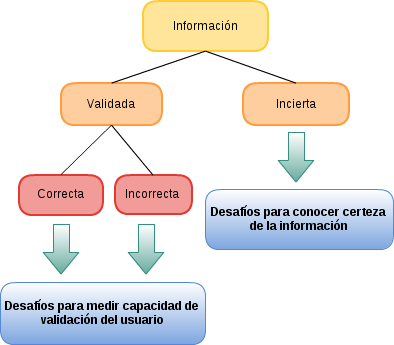
\includegraphics[width=200pt]{./imgs/Info.png}
\caption{Tipos de información y desafíos}
\end{center}
\end{figure}

\begin{itemize}
 \item \textbf{Desafío generado a partir de información validada y correcta:} Si el usuario responde el desafío diciendo que la información es correcta, obtiene algún beneficio, de lo contrario, recibe alguna penalización. De esta forma se verifica la confiabilidad de validar información del usuario.
 \item \textbf{Desafío generado a partir de información validada e incorrecta:} Análogo al anterior, sólo que en este caso el usuario debería responder que la información es incorrecta, de lo contrario, es penalizado.
 \item \textbf{Desafío generado a partir de información incierta:} En este caso, el desafío tiene el objetivo de conocer la correctitud de cierta información aportada por algún usuario. Es por ello, que como resultado de las respuestas de este desafío, y utilizando algún criterio de validación (profundizados en la siguiente sección), finalmente se determinará si la información entregada es correcta o incorrecta, y de esa forma pasará a estar validada.\\
\end{itemize}

De esta forma, en el último caso descrito, hay un traspaso de información incierta a validada, luego de saber si ésta era correcta o incorrecta mediante los desafíos.\\

A continuación se describe un ejemplo del proceso de validación en la aplicación.

\subsection{Proceso de Validación}

En la aplicación final se pretende que exista validación de la ubicación de los lugares, sus tags, y la información de los mismos. En este caso, se mostrará un ejemplo de validación de tags, ya que es la funcionalidad que se quiere obtener en los prototipos a desarrollar durante este trabajo dirigido.\\

Supongamos un usuario, Arturo, se encuentra visitando la Plaza de Armas, y utiliza la aplicación en su móvil. Dentro de las opciones que le muestra el sistema, existe la opción de agregar un tag al lugar, luego, el proceso seguiría de esta forma:\\

\begin{itemize}
 \item Supongamos que en el sistema existe como información validada la relación entre el lugar ''Plaza de Armas`` y los tags ''plaza``, ''estatua`` y ''artistas``.
 \item Arturo agrega el tag ''fuente`` a la Plaza de Armas, ya que vio que había una fuente en ella, y no estaba entre los tags del lugar.
 \item El tag aún no aparece en el sistema, pero es añadido a la Base de Datos como información aún no validada.
 \item Otro usuario, Beatriz, visita la plaza de armas, al usar la aplicación, recibe una tarea de validación en la que se le pregunta si cree que el tag ''fuente`` es un tag válido para Plaza de Armas. Beatriz puede responder que este tag es correcto, incorrecto, o bien, pasar sin responder.
 \item Luego de responder, Beatriz marca como visitada la Plaza de Armas en la aplicación, y aparece un mensaje que le indica que ha ganado 3 puntos de experiencia.
 \item La misma pregunta de validación creada a partir del tag aportado por Arturo, es enviada a varios usuarios que visitan la Plaza de Armas
 \item De acuerdo al criterio de validación escogido, los cuales serán descritos en la siguiente sección, cuando se tenga un número de respuestas razonables, se determina si el tag es correcto o no, dependiendo de las respuestas de los usuarios. En este caso, si el Administrador del sistema observa que el alrededor del 90\% de los usuarios que respondió el desafío del tag ''fuente``, indicaron que era correcto asociarlo a Plaza de Armas, agregará este tag a los tags validados para este lugar.
 \item Por lo tanto, el tag ''fuente'' pasa a ser parte de los tags de Plaza de Armas, luego, pasa a ser información validada, y en este caso, es correcta, y será visible para los usuarios que visiten la Plaza de Armas de ahora en adelante.

\end{itemize}

En el ejemplo descrito, Beatriz recibió una tarea de validación sobre información incierta, aportada por otro usuario. Otro caso posible, hubiese sido que Beatriz recibiera un desafío, por ejemplo, si el tag ``plaza'' es válido para Plaza de Armas. Como es información validada como correcta, si Beatriz responde que la información es correcta, recibirá puntos de experiencia como beneficio, no obstante, en caso de contestar de forma errónea, en este caso, que la relación es incorrecta, perderá puntos de experiencia.\\

\subsection{Criterios de Validación}

Existen dos formas en que la información sea validada en el sistema, ya sea porque un administrador la aprueba como valida, revisando uno a uno las respuestas obtenidas para cada tag, o bien automáticamente valida como correctas o incorrectas todas aquellas que tengan un porcentaje superior al 90\% de respuestas en una de estas dos alternativas.\\

Para el prototipo Alfa desarrollado en el contexto de este trabajo dirigido, sólo se implementará la validación mediante un administrador, eso mediante una interfaz que le permita observar cuantos usuarios han evaluado un tag como correcto(``SI``) o como incorrecto(''NO``):
\begin{figure}[h]
\begin{center}

\includegraphics[width=180pt]{./imgs/TripdroidAdmin.png}
\caption{Menú Administrador}
\end{center}
\end{figure}

\newpage
En la versión Beta a desarrollar se tendrá implementado un caso de validación automática, el cuál es validar como correctos o incorrectos todos los tags que hayan recibido al menos un 90\% de respuestas con esa opción, y tengan por lo menos 10 respuestas entregadas. No obstante, será implementada de manera que debe ser activada por el administrador, es decir, en el menú de administración  existirá la opción de validar automáticamente todos los tags que cumplan esa condición sin la necesidad de revisarlos.\\

\subsection{Beneficios y Penalizaciones}

Para motivar a los usuarios a responder de forma confiable los desafíos, estos deben obtener algo a cambio de resolverlos, en este caso, mayor acceso a información ya validada.\\

En el caso de la aplicación descrita en este informe, para el prototipo Alfa se tendrá desarrollado un sistema de puntaje (experiencia) y niveles por usuario, en el cual, cada vez que un usuario responda una tarea de validación obtiene 3 puntos de experiencia, y al alcanzar cierto número de puntos, asciende de nivel, lo que le permite acceder a más lugares en el mapa. En particular, se tienen definidos lugares que ven todos los usuarios y lugares a los que tienen acceso usuarios en el nivel 2 hacia arriba. Luego, mientras más preguntas sean respondidas, el usuario puede ganar acceso a ver más lugares de la ciudad en el mapa.\\

Para la versión Beta se desea mejorar este sistema de puntaje, verificando la correctitud de la respuesta del usuario para el caso de los desafíos, restándole 3 puntos de experiencia en lugar de sumarlos en caso de que responda en forma errónea.\\

Además, para la versión Beta se implementará el aumentar el número de desafíos cada vez que un usuario responda erróneamente a uno de ellos.\\

\subsection{Consideraciones del Sistema de Validación}

El sistema propuesto para la validación, debe tener contempladas diversas situaciones que pueden ocurrir en el normal uso de la aplicación, o bien, por mal uso de la misma, las cuales pueden afectar la correcta validación de la información, como por ejemplo:\\

\begin{itemize}
\item Que un usuario entregue constantemente información incorrecta y la valide el mismo u otros usuarios que conozca, que un mismo usuario responda varias veces el mismo desafío, que un usuario cree un script para responder desafíos y ganar puntaje, etc.

En el prototipo Beta a desarrollar, para evitar el mal uso de la aplicación, se implementarán tareas de validación basadas en información validada, las que permiten saber si el usuario está validando de forma confiable, además, como se mencionó, una forma de penalización a implementar es aumentar el número de desafíos que reciba el usuario cada vez que quiera visitar un lugar, en caso de haber contestado erróneamente alguna validación, lo que evita que un usuario responda aleatoriamente o mediante un script para ganar puntaje de forma automática.\\

\item Que los usuarios respondan siempre el mismo desafío. Esto es algo normal dentro del uso de la aplicación, y no un mal uso de la misma. Por ejemplo, si uno o más usuarios visitan un mismo lugar a diario, como la universidad, muy probablemente ellos mismos aportaran información y tags sobre ese lugar, y ellos mismos validarán constantemente la información aportada por sus pares, lo que podría ocurrir es que constantemente se les pregunte por el mismo tag, por lo tanto, se tendrían muchas respuestas en el sistema, pero pueden ser todas del mismo usuario. No obstante, para evitar esto se tendrá una relación binaria entre tags y lugares, de modo que no necesariamente se les pregunte por los tags que han sido asociados a ese lugar por otros usuarios, sino que se les pueda preguntar a través de un desafío si un tag cualquiera en el sistema puede corresponder a ese lugar. Esto se implementará de modo que al agregar un nuevo lugar al sistema, automáticamente se agregan desafíos para ese lugar con el resto de los tags almacenados.\\
\end{itemize}

Finalmente, cabe señalar que el objetivo de la aplicación no es garantizar seguridad perfecta dentro de la misma, pero sí la mayor confiabilidad posible de la información existente en ella, por lo cuál el objetivo es buscar la mejor forma de minimizar la información errónea sin alterar demasiado el normal uso de la aplicación de los usuarios. De esta manera, la idea es que un usuario reciba un desafío como máximo en el uso normal de la aplicación, y sólo aumentarán en caso de que responda erróneamente, de modo de no sobrecargarlo con éstos en busca de mayor seguridad.

\subsection{Alternativas de Desarrollo}

A continuación se describen otras consideraciones que se deben tener para el caso de la aplicación descrita en este informe, aunque estas no vayan a ser implementadas en los prototipos :\\

\subsubsection{Automatización de los Criterios de Validación}

A continuación se describen subjetivamente criterios que se pueden aplicar en general para automatizar la validación de información, ya que la forma en que se defina depende en gran medida del tipo de aplicación o del uso de la misma en la práctica, para finalmente poder automatizar los criterios, y así evitar usar una validación centralizada.\\

En el caso de una validación por parte del administrador, éste debe tener conocimiento de las respuestas de los usuarios en un desafío determinado, para poder determinar si valida la información o no, luego, por ejemplo, si cierta información ha sido aprobada como valida por el 99\% de los usuarios que respondieron el desafío, es muy probable que el administrador la acepte como válida, luego, este proceso se puede automatizar. No obstante, el criterio del administrador es útil en casos de que la validación del desafío esté dividida, por ejemplo, si un 60\% de los usuarios cree que cierta información es válida, es una cantidad poco razonable como para automatizar esta respuesta, sin embargo, si se tiene un administrador del sistema, que se sabe que es confiable, se asume que averiguará si el tag corresponde o no antes de aceptarlo como válido en el sistema.\\

Así, en los casos que son claros como el primero mencionado, se puede automatizar la validación. Para esto, se debe establecer algún criterio en el cual se involucre: el número de usuarios que respondieron el desafío, la respuesta que dio al desafío la mayoría de los usuarios (información válida o inválida), y el porcentaje de usuarios que optó por dicha respuesta.\\

Asimismo, también se puede fijar un criterio de acuerdo al número total de usuarios de la aplicación, es decir, si son 1000 usuarios, un 5\% que responda un desafío es razonable, sin embargo, si son 10 mil o 100 mil, probablemente ese porcentaje necesario deba ser menor, debido a que difícilmente 500 o 5000 usuarios distintos visiten un mismo lugar utilizando la aplicación.\\

\subsubsection{Asignar Beneficios y Penalizaciones Según Dificultad}

Como se describió, en los prototipos a desarrollar, los beneficios recibidos por los usuarios son siempre los mismos al responder una tarea de validación.\\

Sin embargo, es bastante razonable que los beneficios o penalizaciones recibidas dependan de la dificultad de la validación, ya que por ejemplo, en el caso de la aplicación a desarrollar, si se tuviesen validaciones sobre los lugares, y ésta consistiera en encontrar un cajero automático que otro usuario señaló que estaba cercano a un lugar, es bastante comprensible que se entregue una respuesta errónea si el usuario efectivamente no pudo encontrar el cajero, pese a que existe. Sin embargo, si se pregunta a un usuario si es correcto el tag ''plaza`` para la Plaza de Armas, asumiendo que es una información ya validada como correcta en el sistema, difícilmente será mal contestada la tarea de validación asociada a este tag, por lo cual se considera razonable penalizar a los usuarios que respondan mal el desafío, ya sea reduciendo su acceso a información en el sistema u otra forma.\\

En general, se puede considerar que un desafío de validar si la ubicación de cierto lugar es correcta es más complejo que un desafío de validar un tag.\\

\subsubsection{Otras Consideraciones de Seguridad}

Otra posibilidad de un mal uso de la aplicación, además de las señaladas, es que un usuario aporte y valide información inválida.\\ Supongamos que un usuario agregue un lugar falso que se encuentra cerca de su casa, o un lugar donde esté constantemente, luego, utilizando otro usuario en la aplicación podría pasar varias veces por el mismo lugar y marcarlo como válido. Una solución a esto, es enviarle el desafío de validar si el lugar existe a un usuario que se encuentre lejano a ese lugar, o que no lo visite habitualmente, dándole la opción de viajar hasta el lugar y luego responder el desafío, el cual, por supuesto, conllevaría un mayor beneficio para el usuario si decide realizarlo. En este caso, se asume que difícilmente un usuario va a viajar para validar un lugar y mentir acerca del mismo, así que se le asocia un mayor beneficio dentro de la evaluación de la validez de la ubicación del lugar, a la respuesta del usuario lejano.\\

\subsubsection{Usuarios Anónimos}

Otra opción a considerar dentro de la aplicación es la de tener usuarios anónimos en ella, es decir, que puedan acceder a ella sin necesidad de registrarse.\\

Para ello, se debe considerar que si un usuario no está registrado, a priori no se almacenará el puntaje u otros beneficios que obtenga, luego, no tendría motivación para validar en forma honesta la información, por lo que hay que decidir como se comportará el sistema de validación respecto a este tipo de usuarios.\\

En los prototipos a entregar se tendrá el acceso restringido solamente a usuarios registrados, sin usuarios anónimos, no obstante, a continuación se explican 3 posibles formas de integrar usuarios anónimos al sistema y cuál es la más adecuada para esta aplicación:\\

\begin{itemize}
 \item \textbf{Ninguno:} Obligar a registrarse para usar la aplicación. No parece una buena idea, ya que el usuario no puede hacerse una idea de qué puede hacer con la aplicación y si le será útil. Además como se vio, existen muchas aplicaciones similares, por lo que lo más probable es que busque otra que no requiera registro.\\
 \item \textbf{Acceso Limitado:} Permitir al usuario anónimo tener acceso a algunas features, sin embargo, sin poder realizar ninguna acción que permita guardar datos relativos a su usuario en el sistema. Es decir, el usuario anónimo en la aplicación podría revisar los lugares que existen en el mapa, y sus tags, sin embargo, no podría marcarlos como visitados ni obtener puntaje, por lo mismo, no tendría sentido que tuviese que responder desafíos ya que tampoco estaría aportando información al sistema.\\
 \item \textbf{Acceso Total:} Los usuarios anónimos tienen acceso completo al sistema, luego, pueden visitar lugares y ganar puntaje a través de los desafíos. Por lo tanto,  para conservar el puntaje y los beneficios obtenidos, deben registrarse en el sistema. Además, es conveniente que por el mismo hecho de no estar registrados, reciben más desafíos al usar la aplicación, y de esta manera, en la aplicación se indique que al registrarse se recibirán menos desafíos.
\end{itemize}

La opción del acceso total es la más razonable para esta aplicación, ya que como se señaló, no darle acceso a usuarios anónimos no es buena idea, debido a que existen alternativas que no requieren registros. Y para el caso del acceso limitado, si bien no tendrán acceso a todo el mapa, el usuario anónimo podría realizar varias acciones sin necesidad de completar desafíos (ya que no tendrían sentido en este caso), y sería extraño para el usuario tener que responderlos una vez registrado.\\

Finalmente, la mayor ventaja de dar acceso total, aunque con mayor número de desafíos a los usuarios anónimos, es que éstos podrán observar todas las capacidades de la aplicación y motivarlos realmente a utilizarla, además de contribuir indirectamente a la misma mediante el control de calidad que efectúen al responder desafíos, o incluso si aportan información que resulta ser validada.\\


\newpage
\section{Planificación Trabajo Dirigido}

Para cumplir los objetivos señalados, la idea es desarrollar el primer prototipo y luego de ello, realizar un estudio de usabilidad del mismo para así elaborar un segundo prototipo basado en las opiniones de los usuarios.\\

Luego, la planificación para efectos del Trabajo Dirigido es la siguiente:\\

\begin{itemize}
\item \textbf{2 - 20 Mayo:} Elaboración Prototipo Alfa, descrito en la siguiente sección.
\item \textbf{6 Junio - 30 Junio:} Encuestar usuarios que utilicen el prototipo y realizar análisis de resultados.
\item \textbf{1 Julio - 10 Julio:} Definir el sistema de validación colaborativa que se espera tener en la aplicación y desarrollar las mejoras más solicitadas por los usuarios luego de la encuesta. (Estas fueron detalles de la interfaz, como destacar más los tags, y principalmente, que los desafíos fueran relativos al lugar que se está visitando).
 \item \textbf{11 Julio - 31 Julio:} Elaborar prototipo Beta basado en los resultados obtenidos. Desarrollando las siguientes funcionalidades:
  \begin{itemize}
  \item \textbf{11 Julio - 17 Julio:} Permitir agregar lugares nuevos al usuario, centrar el mapa en su ubicación actual e indicarla en el mismo. Crear desafíos con tags en el sistema automáticamente cada vez que se agregue un nuevo lugar.
  \item \textbf{18 Julio - 24 Julio:} Agregar tareas de validación basadas en tags ya validados, o de tags que no necesariamente estén relacionados con el lugar. Sistema de suma y resta de puntaje de acuerdo a las respuestas de las validaciones.
  \item \textbf{25 Julio - 31 Julio:} Agregar como penalización que aumente el número de desafíos requeridos para visitar un lugar. Mejorar interfaz de administrador, agregando opción de validar automáticamente desafíos con cierto porcentaje de respuestas iguales. 
  \end{itemize}
\end{itemize}

\newpage
\section{Primer Prototipo (A Mediados del Proyecto)}

\subsection{Propuesta}

Finalmente, la propuesta del prototipo a realizar sería uno que tenga las siguientes características:

\begin{itemize}
\item Al menos 4 lugares identificados en el mapa, de los cuales, por ejemplo, sean 2 que se muestren al inicio al usuario antes que haya resuelto algún desafío.

\item Desarrollar, al menos, el sistema de validación de tags de los lugares, con el objetivo de mostrar un desafío al usuario de prueba.

\item Permitir que el usuario agregue tags a los lugares ya existentes, para probar la validación de los mismos.

\item Además, desarrollar uno de los sistemas de premiación al usuario, se estima como mínimo, el de puntaje por usuario, el cual debe ir desbloqueando lugares para el usuario a medida que este aumente su puntuación.
\end{itemize}

Se estima que con estas mínimas funcionalidades se puede presentar al usuario de prueba un prototipo que represente a grandes rasgos el objetivo de la aplicación y le permita determinar si es simple de entender y usar, y además realizar propuestas sobre como cree que se puede usar la aplicación o aportar nuevas ideas en general.


\subsection{Descripción}

Para efectos del desarrollo, se eligió desarrollar en el Sistema Operativo Android, debido a que era el de más fácil acceso en cuanto a disponibilidad de móviles para desarrollar, y móviles más comumento utilizados por los usuarios.\\

La aplicación tiene un lado servidor y el lado cliente, que corresponde a la aplicación en el equipo.\\

Se describe a continuación el diseño de ambas partes.

\subsubsection{Cliente}

Una aplicación Android se encuentra definida por Actividades (Activity de ahora en adelante), e Intents.\\

Una \textit{Activity} (es decir, una clase de la aplicación que hereda de la clase Activity) se presenta al usuario como una ventana. Esta clase crea una ventana que muestra una interfaz de usuario, vale decir, corresponden a todas las ventanas de una aplicación. \\

Un \textit{Intent} es una clase que permite especificar una Activity a ejecutar, llamando a uno de los métodos de la clase Activity con ese Intent de parámetro.\\

Luego, en cada Activity existen Intents hacia otras actividades. A continuación se muestra un diagrama con las Activities de la aplicación y los Intents reflejados mediante flechas entre las Activities.\\

\begin{figure}[h]
\begin{center}
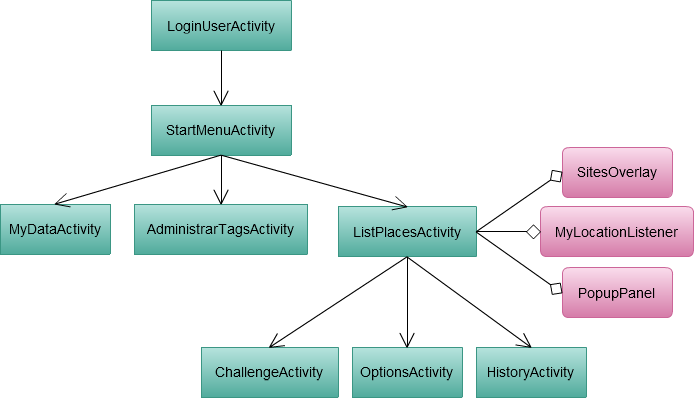
\includegraphics[width=400pt]{./imgs/TripdroidActivities.png}
\caption{Activities de la Aplicación}
\end{center}
\end{figure}

\newpage
Descripción de las Activities:\\

\paragraph{LoginUserActivity:} Contiene formulario para el registro y login de Usuario. Se valida enviando los datos de usuario y password al servidor para comprobar si el usuario existe.


\begin{figure}[h]
\begin{center}
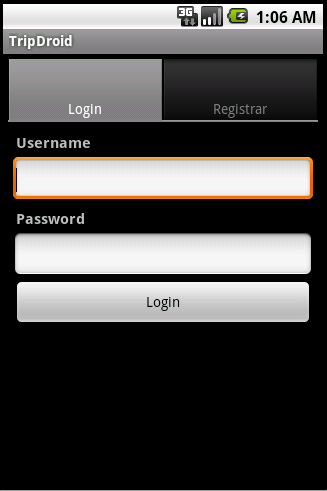
\includegraphics[width=180pt]{./imgs/TripdroidLogin.png}
\caption{Login y Registro}
\end{center}
\end{figure}

\newpage
\paragraph{StartMenuActivity:} Menu inicial que contiene enlaces a los Datos del Usuario, Ver el Mapa, o Administrar en caso de que el usuario sea un administrador.

\begin{figure}[h]
\begin{center}
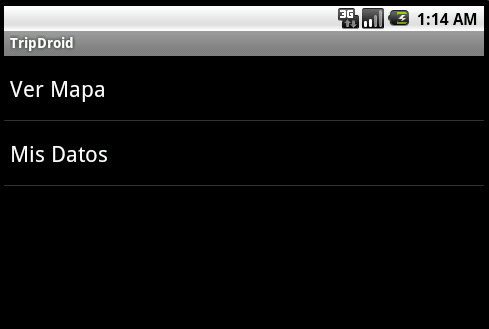
\includegraphics[width=180pt]{./imgs/TripdroidStartMenu.png}
\caption{Menú de Inicio}
\end{center}
\end{figure}

\paragraph{MyDataActivity:} Menú que resume los datos del usuario, su nombre, correo y experiencia.

\begin{figure}[h]
\begin{center}
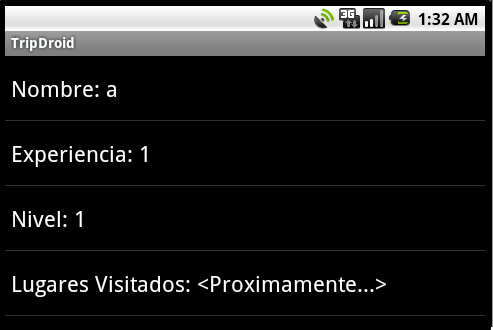
\includegraphics[width=180pt]{./imgs/TripdroidDatos.png}
\caption{Datos del Usuario}
\end{center}
\end{figure}

\newpage
\paragraph{AdministrarTagsActivity:} En caso de que el usuario sea un administrador, tiene acceso a esta actividad, la cual muestra una lista con los tags propuestos por los usuarios, además de los votos que han recibido como correctos o incorrectos para que el administrador pueda ingresarlos al sistema o no.

\begin{figure}[h]
\begin{center}

\includegraphics[width=180pt]{./imgs/TripdroidAdmin.png}
\caption{Validación Tag}
\end{center}
\end{figure}

\paragraph{ListPlacesActivity:} Actividad que carga el Mapa y los lugares que estén cargados en la aplicación, con sus tags e información. El usuario puede visitar o agregar tags a los que se encuentren cercanos a su ubicación actual. Esta actividad funciona mediante las siguientes clases:\\

\begin{itemize}
 \item \textbf{SitesOverlay:} Clase que carga el mapa y los lugares.
 \item \textbf{MyLocationListener:} Thread que lee la ubicación actual del usuario mediante GPS
 \item \textbf{PopupPanel:} Ventana emergente con las coordenadas e información del lugar, y los botones que permiten realizar distintas acciones en el lugar al usuario.
\end{itemize}

\begin{figure}[h]
\begin{center}
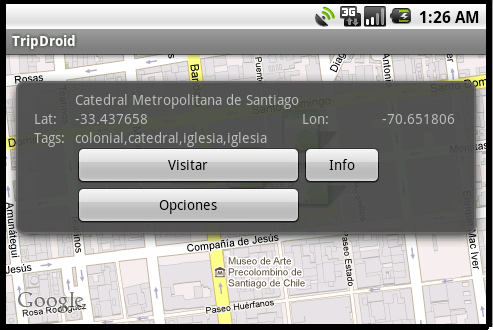
\includegraphics[width=180pt]{./imgs/TripdroidMapaMenu.png}
\caption{Mapa con Lugares}
\end{center}
\end{figure}

\newpage
\paragraph{ChallengeActivity:} Envía un desafío al usuario, en este caso, una pregunta acerca de si es correcta la relación entre un Lugar y un Tag.

\begin{figure}[h]
\begin{center}
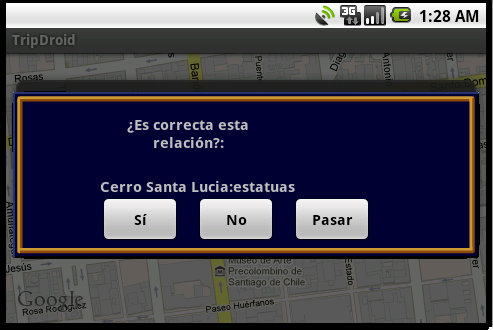
\includegraphics[width=180pt]{./imgs/TripdroidDesafio.png}
\caption{Desafío tipo Tag}
\end{center}
\end{figure}

\paragraph{OptionsActivity:} Aquí el usuario puede aportar datos acerca del Lugar, en el caso del prototipo, sólo puede proponer nuevos tags para el Lugar, que son posteriormente validados mediante desafíos para otros usuarios.

\begin{figure}[h]
\begin{center}
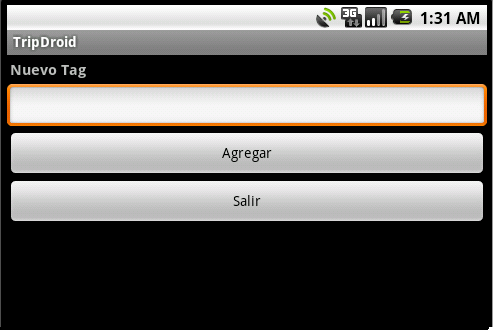
\includegraphics[width=180pt]{./imgs/TripdroidOpciones.png}
\caption{Agregar Tag}
\end{center}
\end{figure}

\paragraph{HistoryActivity:} Aún no desarrollada completamente. Actividad que muestra la historia o más información sobre el lugar.

\newpage
Además, existen otros 2 packages en la aplicación: Utils y Model\\

\paragraph{Model}

Contiene clases que son Objetos que corresponden a las distintas Tablas de la Base de Datos.(Place, User, DesafioTag).\\

\paragraph{Utils}

Contiene clases que se usan para desarrollar funcionalidades de las clases principales.\\

\begin{itemize}
 \item \textbf{InteractiveArrayAdapter:} Clase que adapta los arreglos de las ListView de Android para que tengan un CheckButton.
 \item \textbf{UserSession:} Maneja las sesiones de Usuario, contiene una instancia del objeto correspondiente al usuario actual en la aplicación.
 \item \textbf{WebServiceJSON:} Clase que permite obtener y enviar parámetros en formato de archivo JSON al servidor.
\end{itemize}

\subsubsection{Servidor}

El Servidor de la aplicación corresponde a un servidor gratuito de Google App Engine, donde se tienen los datos de los usuarios, lugares y desafíos y los distintos métodos para obtener dichos datos desde la aplicación cuando se requiera.\\

El modelo de datos es el siguiente:\\

\begin{figure}[h]
\begin{center}
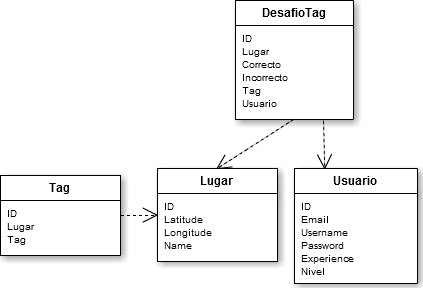
\includegraphics[width=220pt]{./imgs/ModeloDatos.png}
\caption{Agregar Tag}
\end{center}
\end{figure}

Y los métodos que tiene el Servidor son los siguientes: (todos los métodos reciben parámetros vía GET y retornan texto en formato JSON según lo que se requiera)\\

\begin{itemize}
\item \textbf{votaruntag():} Recibe como parámetro un tag y la respuesta del usuario al desafío asociado a ese tag (Sí o No) y le suma un punto al campo ‘correcto’ o ‘incorrecto’ de ese tag según corresponda.

\item \textbf{agregardesafiotag():} Al agregar un nuevo tag, éste método lo recibe como parámetro y crea el desafío asociado a la combinación lugar/tag/usuario, verificando que no exista previamente.

\item \textbf{obtenerdesafiotag():} Retorna un desafío al azar entre todos los desafíos que no hayan sido propuestos por el usuario que invoca el método. Esto es para generar la pregunta de la actividad del desafío.

\item \textbf{obtenertags():} Recibe como parámetro un lugar, y retorna los tags asociados al mismo.

\item \textbf{administrartags():} Retorna una lista de todos los desafíos de tags pendientes, junto con los votos que han recibido.

\item \textbf{agregarnuevotag():} Recibe como parámetro un tag que el administrador haya chequeado como correcto, luego, agrega este tag al lugar correspondiente y borra el desafío asociado a dicho tag.

\item \textbf{registrar():} Recibe como parámetros todos los datos del formulario de registro del usuario, y en caso de no existir un usuario con el mismo username, o email, lo registra en el sistema.

\item \textbf{login():} Recibe como parámetros el username y el password, verifica que la combinación sea correcta y le permite ingresar a la aplicación.

\end{itemize}

\subsection{Instalación}

La aplicación consiste en un archivo llamado ''Tripdroid.apk`` a continuación se describen los pasos a seguir para instalarla, y los requisitos que debe cumplir el equipo.\\

La aplicación ha sido probada en los siguientes equipos:\\

\begin{itemize}
 \item Optimus One P500
 \item Xperia Mini X10
 \item Galaxy Mini S5570
 \item Nexus One
\end{itemize}

\subsubsection{Requisitos para Instalar}

Se debe tener activada la instalación de aplicaciones de orígnes desconocidos en el equipo, en:\\

Configuraciones $\rightarrow$ Aplicaciones $\rightarrow$ Orígenes Desconocidos\\

Además se debe contar con un File Manager para leer el .apk en el equipo, como por ejemplo, el Linda Manager, ya que la aplicación aún no está publicada en el Android Market.\\

\subsubsection{Instalación}

Se debe buscar el .apk en el File Manager y seleccionar la opción de instalarlo en el equipo.\\

Al instalarse, la aplicación solicitará los siguientes permisos:\\

\begin{itemize}
 \item Acceder a Su Ubicación, localización GPS detallada.
 \item Almacenamiento (Modificar o eliminar contenido de la tarjeta de memoria).
 \item Comunicación por Red (Acceso a Internet).
 \item Herramientas del Sistema (Impedir que el teléfono entre en modo inactivo).
\end{itemize}

Se debe aceptar todo, haciendo click en Instalar.

\subsubsection{Requisitos para Utilizar la Aplicación}

Se debe usar internet vía Wi-Fi (es decir, la opción de Red Inalámbrica debe estar habilitada). Y además desactivar el GPS, ya que por ahora la aplicación toma la ubicación actual a traves del Wi-Fi, esto será así al menos para el primer prototipo.

\newpage
\subsection{Prueba con Usuarios}

Luego de elaborar el primer prototipo de la aplicación, éste fue mostrado a los usuarios utilizando un móvil Xperia Mini X10, mediante el cual probaron la aplicación, realizando las siguientes tareas:\\

\begin{itemize}
 \item Registrarse en la aplicación
 \item Visualizar el mapa
 \item Buscar un lugar cercano a su ubicación actual
 \item Visitarlo
 \item Responder un desafío
 \item Agregar un Tag
\end{itemize}


Posteriormente se le realizó una encuesta de usabilidad a los usuarios, donde evaluaron distintas característas en una escala de 1 a 5 (desde "Muy en Desacuerdo" hasta "Muy de Acuerdo"), y luego se permitía entregar feedback libre sobre la aplicación.\\

La encuesta fue realizada a 15 usuarios.\\

\subsubsection{Resultados Encuesta}

La escala fue normalizada de la siguiente forma:

\begin{itemize}
\item Muy en Desacuerdo : 1
\item En desacuerdo: 2
\item Neutro: 3
\item De acuerdo: 4
\item Muy de Acuerdo: 5
\end{itemize}

A continuación se muestran las preguntas de la encuesta en el orden en que fueron realizadas junto con el promedio de las respuestas de los encuestados junto a cada una.\\

\begin{enumerate}
\item La aplicación es fácil de usar \textbf{3,5}
\item Es fácil encontrar la información deseada \textbf{3,3}
\item Las distintas opciones funcionan correctamente \textbf{3,1}
\item Las velocidad de la aplicación es adecuada \textbf{3,4}
\item El uso del color es aceptable \textbf{3,4}
\item El diseño general de la aplicación es apropiado \textbf{3,2}
\item La organización de la información de la aplicación es apropiada \textbf{3,5}
\item El contenido de la aplicación es relevante \textbf{3,2}
\item La interfaz de la aplicación es placentera \textbf{3,2}
\item La aplicación tiene todas las funcionalidades esperadas \textbf{3}
\item La aplicación tiene todas las capacidades esperadas \textbf{3}
\item ¿Cómo califica globalmente la aplicación analizada? \textbf{3,2}

\item Promedio Total: \textbf{3,2}
\end{enumerate}

\newpage
Como se puede observar, todos los resultados están entre 3 y 4, es decir, entre Neutro y De Acuerdo, lo que arroja el siguiente gráfico:\\

\begin{figure}[h]
\begin{center}
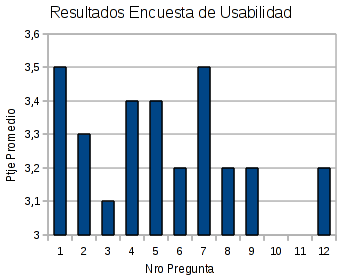
\includegraphics[width=200pt]{./imgs/encuesta.png}
\caption{Promedio obtenido en cada pregunta de la encuesta}
\end{center}
\end{figure}


\subsubsection{Feedback Usuarios}

Comentarios varios de los usuarios que probaron el prototipo y respondieron la encuesta, ordenados por los que se repitieron (o muy similares) más frecuentemente:\\

\begin{itemize}
\item Que los desafíos sean del lugar que visito (9 personas)
\item Permitir agregar nuevos lugares (8 personas)
\item Arreglar el focus del click en la ventana del lugar(8 personas)
\item Que no sea sólo landscape (8 personas)
\item Agregar búsqueda por tags (6 personas)
\item Que estén todos los lugares disponibles y la experiencia sirva para otra cosa (6 personas)
\item Botón para centrar el mapa (6 personas)
\item Tener familia de íconos propios de la app (5 personas)
\item Asociarlo a redes sociales(5 personas)
\item No se distingue bien en el desafío la parte de lugar::tag(4 personas)
\item Poner los Tags en Info en vez de la ventana emergente, o en ambos lugares. (3 personas)
\item Revisar lugares que visité (2 personas)
\item Revisar lugares que visitaron otros usuarios (2 personas)
\item Poner foto del lugare o ver galería de fotos de un lugar (2 personas)
\item Desbloquear ''easter eggs'' al ganar experiencia (2 personas)
\item Ejemplos del relleno en campos de texto
\item Menú Inicial que de Contexto
\item Pasar del registro directo a la app
\item Guardar username y pass
\item Texto de las ventanas emergentes más lento
\end{itemize}

\subsubsection{Análisis de Resultados}

Se puede apreciar que en general la evaluación de la aplicación es entre Neutro y De Acuerdo, más cercana al valor Neutro, lo cuál era esperable, ya que se hizo un prototipo bastante básico para empezar a probar. De hecho, sólo 3 usuarios de los encuestados evaluaron negativamente la aplicación globalmente.\\

En general, el principal problema con que se toparon los usuarios, fue que los desafíos no fueran relacionados directamente con el lugar que visitaban, sin embargo, la gran mayoría no tuvo inconveniente alguno en comprender intuitivamente lo que era el desafío en sí y que se utilizaba para validar, de hecho, varios de ellos mencionaron que era algo similar a lo que hacen varias aplicaciones en distintas redes sociales mientras probaban la aplicación.\\

Por último, se aprecia que la evaluación más baja es en el item ''La aplicación tiene todas las funcionalidades esperadas`` lo cuál es lógico puesto que se trata de un prototipo con el mínimo de funcionalidades. Esto es positivo, ya que los usuarios en general al ver la aplicación preguntaban por funcionalidades que les gustaría que tuviese o que creían que existían, las cuales se pueden ver en el resumen del feedback recibido, y permiten tener una guía para elaborar el segundo prototipo.\\

\newpage
\section{Propuesta Segundo Prototipo (A Fines del Proyecto)}

A raíz de los resultados obtenidos, para un segundo prototipo, el objetivo es tener las siguientes funcionalidades:\\

ToDo: pasar planificación aquí (?)

\newpage
\section{Fases Posteriores}

Fuera del alcance del Trabajo Dirigido, se pretende seguir con el proyecto de la siguiente manera:\\

Luego de terminar con el segundo prototipo, difundir la aplicación para tener un grupo de usuarios utilizándola, y obtener más feedback, en paralelo a ello, continuar con el desarrollo, el cual a mediano o largo plazo puede considerar alguna de las siguiente features a modo de lluvia de ideas:\\

\begin{itemize}
\item Recomendar lugares al usuario de acuerdo a su ubicación actual o lugares que haya visitado.
\item Dibujar sobre el mapa.
\item Permitir que el usuario proponga rutas sobre el mapa.
\item Realizar comentarios y evaluación de los lugares visitados.
\item Permitir agregar otros usuarios como amigos y compartir información personal y/o relativa al uso de la aplicación con ellos.
\item Mostrar el número de personas que ha visitado un lugar, y posiblemente los amigos que han visitado algún lugar al estar cerca de él.
\item Compartir distintas acciones realizadas en la aplicación a través de redes sociales (por ejemplo, el haber visitado algún lugar).
\item Generar mapa con los lugares que he visitado, y la ruta que he seguido de acuerdo al orden de estos.
\item Permitir agregar imágenes de un lugar,y así tener asociada una galería de imágenes al lugar.
\item Que la aplicación avise en caso de que un amigo haya visitado el mismo lugar muy recientemente.
\item Que los usuarios puedan definir capas de lugares, de acuerdo a los tags.
\item Implementar un chat con usuarios que se encuentren en el mismo lugar.
\item Entregar premios a los usuarios de acuerdo al contexto, similar a lo que hace Foursquare, por ejemplo, una medalla en particular para alguien que visite muchos restaurantes
\item Permitir canjear premios por información de otros lugares, o intercambiarlos con otros usuarios
\end{itemize}

Terminar una versión definitiva de la aplicación basada en los resultados de este Trabajo Dirigido y posteriores encuestas a usuarios en las fases siguientes ya descritas.\\

Luego, dar a conocer la aplicación a empresas que apoyen ideas de innovación y les interese apoyar el proyecto (Cursor, CORFO, etc.), o bien buscar trabajos de investigación relacionados con el área donde la aplicación pueda ser útil.\\

En esa misma línea, postular la aplicación al Concurso Kickstart de Innovación http://islae2.cl/.\\

Diseñar, en conjunto con un profesional del área, un plan de negocios, que cubra más o menos la siguiente idea:\\

\paragraph{Plan de Negocios}

La aplicación, para existir, necesita financiar un Servidor donde pueda permanecer alojada la información que utiliza, y personal de alrededor de 5 personas para mantener la aplicación, en cuanto a observar posibles errores que puedan ocurrir y administrar la información que entreguen las personas, en términos de aceptarla o rechazarla de a acuerdo a la cantidad de personas que la hayan evaluado favorablemente.\\

Para obtener el financiamiento, se proponen 3 ideas:\\

\begin{itemize}
 \item Vender espacios para auspicios dentro de la aplicación misma, de acuerdo al número de usuarios que lo clickean, o ven el auspicio en el caso de la aplicación.

 \item También se puede vender datos de información a los usuarios si lo desean, ya sea para activar alguna feature o bien porque desean tener toda la información de la ciudad en caso de que la estén visitando por un breve período de tiempo.

 \item Vender acceso a toda la información de la ciudad a alguien que lo necesite, por ejemplo, para escribir un libro, o bien, generar estadísticas que pueden contribuir a otras instituciones, por ejemplo, el número de personas que visita cada plaza de Santiago puede ser útil de conocer para el Municipio.
\end{itemize}


\end{document}